
\chapter{TCP/IP}
\section{TCP-protokollen}
\subsubsection*{Introduktion til TCP i Embedded Systems}
TCP (Transmission Control Protocol) er en forbindelsesorienteret protokol, der bruges til pålidelig dataoverførsel mellem enheder på et netværk. I modsætning til UDP sikrer TCP, at alle datapakker ankommer i den rigtige rækkefølge og uden tab. Dette gør TCP velegnet til applikationer, hvor dataens integritet og rækkefølge er afgørende, såsom i filoverførsler eller kommunikation med databaser.

\subsubsection*{TCP's Funktionsmåde}
\paragraph{Trevejs-håndtrykket (Three-Way Handshake)}
TCP-forbindelsen etableres gennem en proces kaldet trevejs-håndtrykket. Denne proces sikrer, at både klienten og serveren er synkroniseret og klar til at kommunikere. Processen involverer tre trin:
\begin{enumerate}
	\item \textbf{SYN (Synchronize):} Klienten sender en SYN-pakke til serveren for at anmode om at oprette en forbindelse.
	\item \textbf{SYN-ACK (Synchronize-Acknowledge):} Serveren svarer med en SYN-ACK-pakke, der bekræfter modtagelsen af SYN-pakken og anmoder om at oprette forbindelse til klienten.
	\item \textbf{ACK (Acknowledge):} Klienten sender en ACK-pakke for at bekræfte modtagelsen af serverens SYN-ACK-pakke. Efter dette trin er forbindelsen etableret.
\end{enumerate}
Dette trevejs-håndtryk er en grundlæggende del af TCP, der sikrer pålidelighed i forbindelsen.

\begin{figure}[!h]
	\centering
	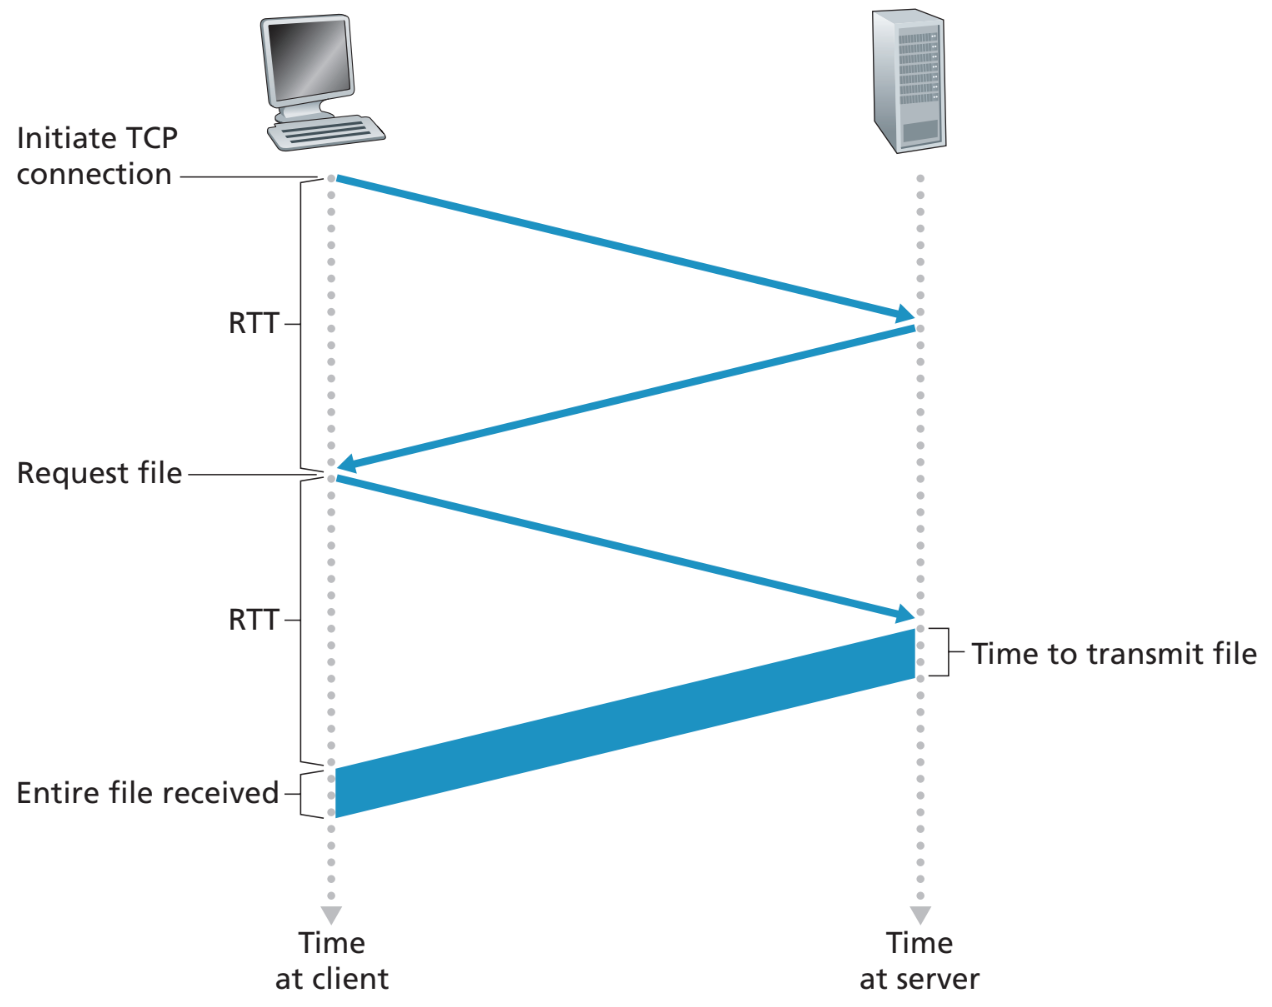
\includegraphics{fig/fig27.png}
	\caption{Three-way handshake}
\end{figure}

\paragraph{Dataoverførsel og Fejlhåndtering}
Når forbindelsen er etableret, opdeler TCP de data, der skal sendes, i segmenter. Hvert segment sendes separat og bekræftes af modtageren ved hjælp af ACK-pakker. Hvis et segment går tabt eller modtages i en forkert rækkefølge, sørger TCP for at sende det igen, indtil modtageren bekræfter det. Dette sikrer, at alle data ankommer i den rigtige rækkefølge og uden tab.
\newline\newline\noindent
TCP bruger også en mekanisme kaldet "flow control" for at sikre, at modtageren ikke bliver overvældet af for mange data ad gangen. Dette gør TCP velegnet til applikationer, hvor stabil og ordnet dataoverførsel er nødvendig.

\paragraph{Brug af TCP i Embedded Systems}
I indlejrede systemer bruges TCP ofte til applikationer, hvor pålidelighed er afgørende, såsom i dataoverførsler mellem en IoT-enhed og en central server. For eksempel kan en sensor, der sender kritiske data til en cloud-server, bruge TCP for at sikre, at dataene ankommer uden fejl eller tab.

\paragraph{Sikkerhed i TCP}
For at beskytte data under overførsel kan TCP kombineres med TLS (Transport Layer Security), som giver kryptering og beskytter mod aflytning og manipulation. Dette er især vigtigt i applikationer, hvor følsomme data overføres over internettet.

\subsubsection{Integration af ESP32 med TCP}
I dette afsnit beskrives de nødvendige trin for at integrere ESP32 med TCP:

\begin{enumerate}
	\item \textbf{Inkluder nødvendige biblioteker}
	\begin{lstlisting}[language=C++, caption=Syntaks]
		#include <WiFi.h>       // WiFi library for ESP32
	\end{lstlisting}
	\noindent Denne linje inkluderer det nødvendige bibliotek for WiFi-forbindelse på ESP32.
	
	\item \textbf{Definer WiFi og TCP-oplysninger}
	\begin{lstlisting}[language=C++, caption=Syntaks]
		const char* ssid = "your_network_name";   // WiFi SSID
		const char* password = "your_password";   // WiFi password
		const char* serverAddress = "server_address"; // TCP server IP address
		const int serverPort = 8080;              // TCP server port
	\end{lstlisting}
	\noindent Her defineres netværksnavnet og adgangskoden til dit WiFi-netværk samt TCP-serverens IP-adresse og port.
	
	\item \textbf{Opret WiFi klient og TCP forbindelse}
	\begin{lstlisting}[language=C++, caption=Syntaks]
		WiFiClient client;  // Create WiFi client object
	\end{lstlisting}
	\noindent Dette skaber et klientobjekt til at styre TCP-forbindelsen.
	
	\item \textbf{Initialiser WiFi-forbindelsen i Setup}
	\begin{lstlisting}[language=C++, caption=Syntaks]
		void setup() {
			Serial.begin(115200); // Start serial communication
			WiFi.begin(ssid, password); // Connect to WiFi
			while (WiFi.status() != WL_CONNECTED) {
				delay(1000); // Wait until connected
				Serial.println("Connecting to WiFi...");
			}
			Serial.println("Connected to WiFi");
		}
	\end{lstlisting}
	\noindent I setup-funktionen initialiseres WiFi-forbindelsen.
	
	\item \textbf{Eksempel på TCP dataoverførsel i Loop}
	\begin{lstlisting}[language=C++, caption=Syntaks]
		void loop() {
			if (!client.connected()) {
				Serial.println("Connecting to server...");
				client.connect(serverAddress, serverPort); // Connect to TCP server
				Serial.println("Connected to server!");
			}
			
			// Send data to the server
			client.println("Hello, Server!");
			
			// Receive data from the server
			while (client.available()) {
				String line = client.readStringUntil('\r');
				Serial.print(line);
			}
			
			delay(10000); // Wait 10 seconds before the next update
		}
	\end{lstlisting}
	Dette eksempel viser, hvordan ESP32 kan sende en besked til en TCP-server og modtage et svar.
	
	\item \textbf{Eksempel på TCP-server på ESP32}
	\begin{lstlisting}[language=C++, caption=Syntaks]
		WiFiServer server(serverPort); // Create a TCP server object
		
		void setup() {
			Serial.begin(115200); // Start serial communication
			WiFi.begin(ssid, password); // Connect to WiFi
			while (WiFi.status() != WL_CONNECTED) {
				delay(1000); // Wait until connected
				Serial.println("Connecting to WiFi...");
			}
			Serial.println("Connected to WiFi");
			
			server.begin(); // Start the server
		}
		
		void loop() {
			WiFiClient client = server.available(); // Check if a client has connected
			if (client) {
				String request = client.readStringUntil('\r');
				Serial.println(request);
				client.flush();
				
				// Handle the client's request
				client.println("HTTP/1.1 200 OK");
				client.println();
				client.stop(); // Close the connection
			}
		}
	\end{lstlisting}
	Dette eksempel viser, hvordan ESP32 kan fungere som en TCP-server, modtage forbindelser fra klienter og sende svar.
\end{enumerate}
\noindent Denne procedure skitserer trin for trin, hvordan ESP32 kan integreres med TCP-protokollen for at kommunikere effektivt i et IoT-miljø. TCP er ideelt til brug i situationer, hvor pålidelig og ordnet dataoverførsel er nødvendig, såsom i applikationer, der kræver en høj grad af dataintegritet.


\chapter{UDP}
\section{UDP-protokollen}
\subsubsection*{Introduktion til UDP i Embedded Systems}
UDP (User Datagram Protocol) er en letvægts, forbindelsesløs kommunikationsprotokol, der anvendes på tværs af netværk til hurtig og effektiv dataoverførsel. I modsætning til TCP (Transmission Control Protocol) giver UDP ingen garantier for levering, rækkefølge eller beskyttelse mod duplikation, hvilket gør det hurtigere, men mindre pålideligt. Disse egenskaber gør UDP velegnet til applikationer, hvor hurtig dataoverførsel er vigtigere end pålidelighed, såsom i streaming eller sensor dataopsamling i indlejrede systemer.

\paragraph{Grundlæggende Funktionsmåde}
UDP fungerer ved at sende datagrammer, som er selvstændige pakker af data, til modtageren. Hver pakke behandles uafhængigt, og der er ingen håndtryk eller forbindelsesoprettelse mellem afsender og modtager, hvilket resulterer i minimal protokoloverhead og hurtigere kommunikation.

\paragraph{Unicast, Multicast og Broadcast}
UDP understøtter forskellige kommunikationstyper, herunder unicast, multicast og broadcast, som hver især er velegnet til forskellige typer af netværksapplikationer:

\begin{itemize}
	\item \textbf{Unicast:} I unicast kommunikation sendes data fra én afsender til én modtager. Dette er den mest almindelige form for kommunikation, hvor data leveres direkte til en specifik enhed.
	\item \textbf{Multicast:} Multicast tillader en enkelt afsender at sende data til flere udvalgte modtagere på én gang. Dette er effektivt i applikationer som streaming, hvor flere enheder skal modtage den samme information samtidig.
	\item \textbf{Broadcast:} I broadcast sendes data fra én afsender til alle enheder i et netværk. Dette bruges ofte i scenarier, hvor en besked skal nå alle tilgængelige enheder, som f.eks. i netværksopdagelse.
\end{itemize}

\paragraph{Fordele i Embedded Systems}
UDP's lette natur og hurtige\\ overførselshastighed gør det særligt velegnet til indlejrede systemer, hvor der kan være behov for at sende små mængder data hurtigt uden behov for bekræftelse. Dette gør det ideelt til real-time applikationer og enkle sensor-netværk.

\paragraph{Sikkerhed}
Da UDP ikke har indbyggede mekanismer til sikring af data, anbefales det at bruge UDP sammen med sikkerhedsprotokoller som DTLS (Datagram Transport Layer Security) for at beskytte data mod aflytning og manipulation.

\subsubsection{Integration af ESP32 med UDP}

Nedenstående kode viser, hvordan man integrerer ESP32 med UDP-protokollen. Koden omfatter opsætning af WiFi-forbindelse og både afsendelse og modtagelse af UDP-pakker.

\begin{lstlisting}[language=C++, caption=ESP32 integration med UDP]
	#include <WiFi.h>       // WiFi library for ESP32
	#include <WiFiUdp.h>    // UDP library for ESP32
	
	// WiFi og UDP konfigurationer
	const char* ssid = "your_network_name";   // WiFi SSID
	const char* password = "your_password";   // WiFi password
	const char* udp_server = "server_address"; // UDP server IP address
	const unsigned int udp_port = 12345;       // UDP server port
	
	WiFiUDP udpClient;  // Opret UDP klient objekt
	
	void setup() {
		Serial.begin(115200); // Start seriel kommunikation
		WiFi.begin(ssid, password); // Forbind til WiFi netværket
		while (WiFi.status() != WL_CONNECTED) {
			delay(1000); // Vent indtil forbindelsen er etableret
			Serial.println("Connecting to WiFi...");
		}
		Serial.println("Connected to WiFi");
	}
	
	void loop() {
		// Afsendelse af UDP pakke til serveren
		udpClient.beginPacket(udp_server, udp_port); // Start UDP pakke
		udpClient.print("Hello, UDP Server!"); // Tilføj besked til pakken
		udpClient.endPacket(); // Send UDP pakke
		
		delay(5000); // Vent 5 sekunder før næste pakke sendes
		
		// Modtagelse af UDP pakker fra serveren
		int packetSize = udpClient.parsePacket(); // Tjek for indkommende pakke
		if (packetSize) {
			char incomingPacket[255];
			int len = udpClient.read(incomingPacket, 255); // Læs pakken ind i buffer
			if (len > 0) {
				incomingPacket[len] = '\0'; // Null-terminer streng
			}
			Serial.print("Received UDP packet: ");
			Serial.println(incomingPacket); // Print modtaget pakke
		}
		
		delay(1000); // Vent 1 sekund før næste tjek
	}
\end{lstlisting}
Denne kode implementerer UDP-kommunikation på en ESP32-enhed. Den viser, hvordan man sender en simpel besked til en UDP-server og modtager data fra serveren. Ved at bruge WiFiUdp-biblioteket kan ESP32 kommunikere over UDP-protokollen, hvilket er ideelt til applikationer, der kræver hurtig og effektiv dataoverførsel, hvor levering af data ikke nødvendigvis skal bekræftes.




\chapter{Modbus}
\section{Modbus-protokollen}

\subsection{Introduktion til Modbus i Embedded Systems}
Modbus er en kommunikationsprotokol oprindeligt udviklet af Modicon (nu Schneider Electric) i slutningen af 1970'erne til brug i industrielt udstyr. Protokollen er blevet en industri-standard for kommunikation i industrielle systemer og er blevet adopteret bredt på grund af dens enkelhed og pålidelighed. Modbus anvendes ofte i indlejrede systemer, især hvor der er behov for kommunikation mellem mikrocontrollere, sensorer, aktuatorer og andre enheder over serielle forbindelser som RS-485 eller over TCP/IP.

\paragraph{Grundlæggende Funktionsmåde}
Modbus fungerer som en master/slave-protokol, hvor en master-enhed (f.eks. en PLC eller mikrocontroller) kommunikerer med en eller flere slave-enheder. Masteren initierer anmodninger, og slaverne reagerer på disse anmodninger. Modbus understøtter forskellige datatyper som coils, discrete inputs, input registers og holding registers, som kan bruges til at læse eller skrive data.

\paragraph{Modbus Function Codes}
Modbus-protokollen definerer forskellige funktionelle koder (function codes) for at udføre specifikke operationer. De mest almindelige funktioner inkluderer:
\begin{itemize}
	\item \textbf{01 - Read Coils}: Læser status af coils (0 eller 1), som er binære udgange, der kan tændes eller slukkes.
	\item \textbf{02 - Read Discrete Inputs}: Læser status af discrete inputs (0 eller 1), som er binære indgange.
	\item \textbf{03 - Read Holding Registers}: Læser værdien af holding registers, som normalt er brugt til at gemme outputdata.
	\item \textbf{04 - Read Input Registers}: Læser værdien af input registers, som normalt er brugt til at gemme inputdata.
	\item \textbf{05 - Write Single Coil}: Skriver en værdi til en enkelt coil.
	\item \textbf{06 - Write Single Register}: Skriver en værdi til et enkelt holding register.
	\item \textbf{15 - Write Multiple Coils}: Skriver værdier til flere coils.
	\item \textbf{16 - Write Multiple Registers}: Skriver værdier til flere holding registers.
\end{itemize}

\paragraph{Data Typer i Modbus}
Modbus definerer flere datatyper, som kan bruges til at interagere med enheder:
\begin{itemize}
	\item \textbf{Coils (0X)}: En coil er en binær output, som kan tændes (1) eller slukkes (0).
	\item \textbf{Discrete Inputs (1X)}: En discrete input er en binær input, som kan være høj (1) eller lav (0).
	\item \textbf{Input Registers (3X)}: Input registers er 16-bit værdier, der typisk bruges til at læse analoge inputdata.
	\item \textbf{Holding Registers (4X)}: Holding registers er 16-bit værdier, der typisk bruges til at gemme outputdata eller konfigurationer.
\end{itemize}

\paragraph{Fordele i Embedded Systems}
Modbus er meget effektiv i indlejrede systemer, hvor stabil kommunikation mellem enheder er nødvendig. Protokollen understøtter både seriel og TCP/IP kommunikation, hvilket gør den fleksibel til mange forskellige typer applikationer.

\paragraph{Sikkerhed}
Modbus i sin grundform tilbyder ikke nogen indbygget sikkerhed. For at sikre Modbus-kommunikation kan den dog køres over sikre transportlag som TLS, eller netværket kan sikres via VPN.

\subsubsection*{Integration af ESP32 med Modbus}
I dette afsnit beskrives de nødvendige trin for at integrere ESP32 med Modbus:

\begin{lstlisting}[language=C++, caption=Integration af ESP32 med Modbus]
	#include <WiFi.h>        // WiFi library for ESP32
	#include <ModbusIP_ESP8266.h> // Modbus TCP library for ESP32
	
	// WiFi configurations
	const char* ssid = "your_network_name";   // WiFi SSID
	const char* password = "your_password";   // WiFi password
	
	// Create Modbus server object
	ModbusIP mb;
	
	void setup() {
		Serial.begin(115200); // Start serial communication
		WiFi.begin(ssid, password); // Connect to WiFi
		
		// Wait for WiFi connection
		while (WiFi.status() != WL_CONNECTED) {
			delay(1000); 
			Serial.println("Connecting to WiFi...");
		}
		Serial.println("Connected to WiFi");
		
		mb.server();  // Start Modbus TCP server
	}
	
	void loop() {
		mb.task();  // Process incoming Modbus requests
		
		// Example: Update a holding register at address 0x0001 with the value 1234
		mb.Hreg(0x0001, 1234);
		
		delay(1000);  // Delay before the next operation
	}
\end{lstlisting}
Denne kode integrerer ESP32 med Modbus-protokollen og samler alle nødvendige funktioner, herunder WiFi-forbindelse, samt læsning og skrivning af coils og registre via Modbus, i én enkelt kodeblok. Dette sikrer robust og pålidelig kommunikation med Modbus-slaver, hvilket er afgørende i industrielle applikationer.	

\chapter{MQTT}
\section{MQTT-protokollen}
\subsubsection*{Introduktion til MQTT i Embedded Systems}
MQTT (Message Queue Telemetry Transport) er en letvægts, publikations- og abonnementsbaseret beskedprotokol, der er designet til at være effektiv og strømlinet, hvilket gør den ideel til brug i Embedded Systems. Dette gør den til en populær protokol indenfor IoT-området, hvor netværksbåndbredde og batteristrøm kan være begrænset.

\paragraph{Grundlæggende Funktionsmåde}
MQTT fungerer på en klient-server-model, hvor klienten kommunikerer med en mægler (broker). Klienter kan abonnere på emner (topics), og når en besked er offentliggjort på et emne af en anden klient, videresender mægleren beskeden til alle abonnenter på det pågældende emne.

\paragraph{QoS (Quality of Service)}
MQTT understøtter forskellige serviceniveauer, kaldet QoS. Disse niveauer bestemmer, hvordan og hvor ofte beskeder sendes:
\begin{itemize}
	\item \textbf{QoS 0}: "Højst én gang" - Beskeden sendes en enkelt gang uden bekræftelse.
	\item \textbf{QoS 1}: "Mindst én gang" - Beskeden sendes og bekræftes, men kan modtages mere end én gang.
	\item \textbf{QoS 2}: "Nøjagtigt én gang" - Beskeden sendes og bekræftes, så modtageren får den nøjagtigt én gang.
\end{itemize}

\paragraph{Fordel i Embedded Systems}
MQTT's letvægts natur og evne til at håndtere ustabile forbindelser gør den særligt velegnet til indlejrede systemer, hvor ressourcer kan være begrænsede. Derudover er dets publikations- og abonnementsmodel egnet til enheder, der kommunikerer over netværk med lav båndbredde.

\paragraph{Sikkerhed}
Selvom MQTT ikke i sig selv tilbyder avancerede sikkerhedsfunktioner, kan det kombineres med sikre transportlag som TLS for at tilbyde en sikker kommunikationskanal.

Dette afsnit giver en oversigt over MQTT og dens egenskaber, som gør den ideel til Embedded Systems. Det dækker grundlæggende funktioner, QoS-niveauer, fordelene ved brug i Embedded Systems og sikkerhedsaspekter.

\subsubsection{Integration af ESP32 med MQTT}

I dette afsnit beskrives de nødvendige trin for at integrere ESP32 med MQTT:

\begin{enumerate}
	\item \textbf{Inkluder nødvendige biblioteker}
	\begin{lstlisting}[language=C++, caption=Syntaks]
		#include <WiFi.h>
		#include <PubSubClient.h>
	\end{lstlisting}
	Disse linjer inkluderer de nødvendige biblioteker for WiFi-forbindelse og MQTT-klient.
	
	\item \textbf{Definer WiFi og MQTT-oplysninger}
	\begin{lstlisting}[language=C++, caption=Syntaks]
		const char* ssid = "your_network_name"; // WiFi SSID
		const char* password = "your_password"; // WiFi password
		const char* mqtt_server = "broker_address"; // MQTT broker address
	\end{lstlisting}
	Her defineres netværksnavnet og adgangskoden til dit WiFi-netværk samt MQTT-brokerens adresse.
	
	\item \textbf{Opret WiFiClient og PubSubClient}
	\begin{lstlisting}[language=C++, caption=Syntaks]
		WiFiClient espClient; // Create a WiFi client object
		PubSubClient client(espClient); // Create a PubSub client object
	\end{lstlisting}
	Dette skaber klientobjekter til at styre WiFi- og MQTT-forbindelserne.
	
	\item \textbf{Definer MQTT Reconnect-funktion}
	\begin{lstlisting}[language=C++, caption=Syntaks]
		void reconnect() {
			while (!client.connected()) {
				Serial.println("Connecting to MQTT..."); // Attempt to connect to MQTT broker
				if (client.connect("ESP32Client")) { // MQTT client ID
					Serial.println("Connected to MQTT!"); // Success message
				} else {
					delay(5000); // Wait before retrying
				}
			}
		}
	\end{lstlisting}
	Denne funktion forsøger at forbinde til MQTT-brokeren, indtil forbindelsen er etableret.
	
	\item \textbf{Initialiser WiFi-forbindelsen og MQTT i Setup}
	\begin{lstlisting}[language=C++, caption=Syntaks]
		void setup() {
			Serial.begin(115200); // Start serial communication
			WiFi.begin(ssid, password); // Connect to WiFi
			while (WiFi.status() != WL_CONNECTED) {
				delay(1000); // Wait until connected
				Serial.println("Connecting to WiFi...");
			}
			Serial.println("Connected to WiFi");
			client.setServer(mqtt_server, 1883); // Set MQTT broker and port
			reconnect(); // Connect to MQTT broker
		}
	\end{lstlisting}
	I setup-funktionen initialiseres forbindelsen til WiFi-netværket og MQTT-brokeren.
	
	\item \textbf{Publiser og abonner på emner i Loop}
	\begin{lstlisting}[language=C++, caption=Syntaks]
		void loop() {
			if (!client.connected()) {
				reconnect(); // Ensure connection to MQTT broker
			}
			client.loop(); // Maintain MQTT connection
			client.publish("topic/path", "Hello from ESP32!"); // Publish a message
			delay(5000); // Delay before next message
			client.subscribe("another/topic/path"); // Subscribe to a topic
		}
	\end{lstlisting}
	I loop-funktionen sikres forbindelsen til MQTT-brokeren, og koden til at publisere og abonnere på emner placeres her.
\end{enumerate}
Denne procedure skitserer trin for trin, hvordan ESP32 kan integreres med MQTT for at sende og modtage beskeder via en broker. Dette kan være fundamentet for forskellige IoT-applikationer, hvor enheder skal kommunikere med hinanden over internettet.

\chapter{HTTP}
\section{HTTP-protokollen}

\subsection*{Introduktion til HTTP i Embedded Systems}
HTTP (HyperText Transfer Protocol) er en protokol, der bruges til at kommunikere over internettet. Den er især nyttig i indlejrede systemer, som f.eks. ESP32, til at sende og modtage data fra servere og andre enheder. Ved at udnytte HTTP kan ESP32 kommunikere med webservices, fjernservere og andre netværksenheder, hvilket gør det muligt at indsamle data fra sensorer, styre aktuatorer og meget mere.

\subsection*{Opsætning og Krav}

\textbf{Hardwarekrav}
\begin{itemize}
	\item \textbf{ESP32 Board:} ESP32 er en kraftfuld mikrocontroller med indbygget WiFi og Bluetooth, ideel til IoT-projekter, hvor der er behov for trådløs kommunikation.
	\item \textbf{Power Supply:} ESP32 kræver en strømforsyning på 3.3V. En USB-kabel, der er forbundet til en computer eller et 3.3V batteri, kan bruges.
	\item \textbf{WiFi Access:} Da HTTP-kommunikation kræver internetadgang, skal ESP32 have adgang til et stabilt WiFi-netværk.
	\item \textbf{Optional External Hardware:} Afhængig af projektet kan yderligere sensorer, aktuatorer eller displays være nødvendige.
\end{itemize}

\textbf{Softwarekrav}
\begin{itemize}
	\item \textbf{Development Environment:} ESP32 kan programmeres ved hjælp af Arduino IDE eller PlatformIO. Disse udviklingsmiljøer skal installeres på din computer.
	\item \textbf{ESP32 Drivers:} For at få ESP32 til at arbejde med Arduino IDE eller PlatformIO skal du installere de nødvendige drivere og biblioteker.
	\item \textbf{HTTP and JSON Libraries:} For at arbejde med HTTP-protokollen og REST API'er skal du inkludere specifikke biblioteker, som \texttt{HTTPClient} til HTTP-kommunikation og \texttt{ArduinoJson} til JSON-parsing.
\end{itemize}

\subsection*{HTTP Requests med ESP32}

Denne sektion forklarer, hvordan du opretter HTTP-requests med ESP32 til at interagere med servere og webservices. Vi vil gennemgå de fire mest almindelige HTTP-metoder: POST, PUT, GET og DELETE.

\subsubsection*{POST Request}
En POST-request bruges til at sende data til en server for at oprette en ny ressource. Dataene sendes i anmodningens body, og serveren opretter en ny ressource baseret på de modtagne data.

\begin{enumerate}
	\item \textbf{Inkluder nødvendige biblioteker:}
	\begin{lstlisting}[language=C++, caption=Include necessary libraries]
		#include <WiFi.h>
		#include <HTTPClient.h>
	\end{lstlisting}
	Disse linjer inkluderer de nødvendige biblioteker for WiFi-forbindelse og HTTP-klient.
	
	\item \textbf{Definer WiFi-oplysninger:}
	\begin{lstlisting}[language=C++, caption=Define WiFi credentials]
		const char* ssid = "your_network_name";
		const char* password = "your_password";
	\end{lstlisting}
	Her defineres netværksnavnet og adgangskoden til dit WiFi-netværk.
	
	\item \textbf{Initialiser WiFi-forbindelsen i \texttt{setup()}:}
	\begin{lstlisting}[language=C++, caption=Initialize WiFi connection in setup()]
		void setup() {
			Serial.begin(115200);
			WiFi.begin(ssid, password);
			while (WiFi.status() != WL_CONNECTED) {
				delay(1000);
				Serial.println("Connecting to WiFi...");
			}
			Serial.println("Connected to WiFi");
		}
	\end{lstlisting}
	I \texttt{setup()}-funktionen initialiseres forbindelsen til WiFi-netværket, og programmet venter, indtil forbindelsen er etableret.
	
	\item \textbf{Opret HTTP-forbindelse i \texttt{loop()}:}
	\begin{lstlisting}[language=C++, caption=Create HTTP connection in loop()]
		void loop() {
			if(WiFi.status() == WL_CONNECTED) {
				HTTPClient http;
				
				http.begin("http://yourNodeRedServerIP:1880/postdata"); // Specify the URL
				http.addHeader("Content-Type", "application/x-www-form-urlencoded"); // Set content type
				
				String postData = "key1=value1&key2=value2"; // Your POST data
				
				int httpResponseCode = http.POST(postData);
				
				if(httpResponseCode>0){
					String response = http.getString();
					Serial.println(response);
				}
				else {
					Serial.print("Error sending POST: ");
					Serial.println(httpResponseCode);
				}
				
				http.end(); // Free resources
			}
			
			delay(10000); // Wait 10 seconds before next update
		}
	\end{lstlisting}
	Denne kode sender en POST-anmodning til din Node-RED-server med dataene \texttt{"key1=value1\&key2=value2"} og udskriver serverens svar i Serial Monitor.
\end{enumerate}

\subsubsection*{PUT Request}
En PUT-request bruges til at opdatere en eksisterende ressource eller oprette en ny ressource, hvis den ikke findes. Dataene sendes til en specifik URL, hvor ressourcen opdateres eller oprettes.

\begin{enumerate}
	\item \textbf{Inkluder nødvendige biblioteker:}
	\begin{lstlisting}[language=C++, caption=Include necessary libraries]
		#include <WiFi.h>
		#include <HTTPClient.h>
	\end{lstlisting}
	
	\item \textbf{Definer WiFi-oplysninger:}
	\begin{lstlisting}[language=C++, caption=Define WiFi credentials]
		const char* ssid = "your_network_name";
		const char* password = "your_password";
	\end{lstlisting}
	
	\item \textbf{Initialiser WiFi-forbindelsen i \texttt{setup()}:}
	\begin{lstlisting}[language=C++, caption=Initialize WiFi connection in setup()]
		void setup() {
			Serial.begin(115200);
			WiFi.begin(ssid, password);
			while (WiFi.status() != WL_CONNECTED) {
				delay(1000);
				Serial.println("Connecting to WiFi...");
			}
			Serial.println("Connected to WiFi");
		}
	\end{lstlisting}
	
	\item \textbf{Opret HTTP-forbindelse i \texttt{loop()}:}
	\begin{lstlisting}[language=C++, caption=Create HTTP connection in loop()]
		void loop() {
			if(WiFi.status() == WL_CONNECTED) {
				HTTPClient http;
				http.begin("http://yourNodeRedServerIP:1880/putdata"); // Specify the URL
				http.addHeader("Content-Type", "application/x-www-form-urlencoded"); // Set content type
				
				String putData = "key1=value1&key2=value2"; // Your PUT data
				
				int httpResponseCode = http.PUT(putData); // Send PUT request
				
				if(httpResponseCode>0){
					String response = http.getString();
					Serial.println(response);
				}
				else {
					Serial.print("Error sending PUT: ");
					Serial.println(httpResponseCode);
				}
				
				http.end(); // Free resources
			}
			
			delay(10000); // Wait 10 seconds before next update
		}
	\end{lstlisting}
	Denne kode sender en PUT-anmodning til din Node-RED-server med dataene \texttt{"key1=value1\&key2=value2"} og udskriver serverens svar i Serial Monitor.
\end{enumerate}

\subsubsection*{GET Request}
En GET-request bruges til at anmode om data fra en server. Dataene returneres som svar på anmodningen, og GET-metoden inkluderer ingen data i anmodningens body.

\begin{enumerate}
	\item \textbf{Inkluder nødvendige biblioteker:}
	\begin{lstlisting}[language=C++, caption=Include necessary libraries]
		#include <WiFi.h>
		#include <HTTPClient.h>
	\end{lstlisting}
	
	\item \textbf{Definer WiFi-oplysninger:}
	\begin{lstlisting}[language=C++, caption=Define WiFi credentials]
		const char* ssid = "your_network_name";
		const char* password = "your_password";
	\end{lstlisting}
	
	\item \textbf{Initialiser WiFi-forbindelsen i \texttt{setup()}:}
	\begin{lstlisting}[language=C++, caption=Initialize WiFi connection in setup()]
		void setup() {
			Serial.begin(115200);
			WiFi.begin(ssid, password);
			while (WiFi.status() != WL_CONNECTED) {
				delay(1000);
				Serial.println("Connecting to WiFi...");
			}
			Serial.println("Connected to WiFi");
		}
	\end{lstlisting}
	
	\item \textbf{Foretag HTTP GET-request i \texttt{loop()}:}
	\begin{lstlisting}[language=C++, caption=Create HTTP connection in loop()]
		void loop() {
			if(WiFi.status() == WL_CONNECTED) {
				HTTPClient http;
				
				http.begin("http://yourServerIP:1880/getdata"); // Specify the URL
				
				int httpResponseCode = http.GET();
				
				if(httpResponseCode>0){
					String response = http.getString();
					Serial.println(response);
				}
				else {
					Serial.print("Error sending GET: ");
					Serial.println(httpResponseCode);
				}
				
				http.end(); // Free resources
			}
			
			delay(10000); // Wait 10 seconds before next update
		}
	\end{lstlisting}
	Denne kode sender en GET-anmodning til din server og udskriver serverens svar i Serial Monitor.
\end{enumerate}

\subsubsection*{DELETE Request}
En DELETE-request bruges til at anmode om, at en ressource bliver fjernet fra serveren.

\begin{enumerate}
	\item \textbf{Inkluder nødvendige biblioteker:}
	\begin{lstlisting}[language=C++, caption=Include necessary libraries]
		#include <WiFi.h>
		#include <HTTPClient.h>
	\end{lstlisting}
	
	\item \textbf{Definer WiFi-oplysninger:}
	\begin{lstlisting}[language=C++, caption=Define WiFi credentials]
		const char* ssid = "your_network_name";
		const char* password = "your_password";
	\end{lstlisting}
	
	\item \textbf{Initialiser WiFi-forbindelsen i \texttt{setup()}:}
	\begin{lstlisting}[language=C++, caption=Initialize WiFi connection in setup()]
		void setup() {
			Serial.begin(115200);
			WiFi.begin(ssid, password);
			while (WiFi.status() != WL_CONNECTED) {
				delay(1000);
				Serial.println("Connecting to WiFi...");
			}
			Serial.println("Connected to WiFi");
		}
	\end{lstlisting}
	
	\item \textbf{Foretag HTTP DELETE-request i \texttt{loop()}:}
	\begin{lstlisting}[language=C++, caption=Create HTTP connection in loop()]
		void loop() {
			if(WiFi.status() == WL_CONNECTED) {
				HTTPClient http;
				
				http.begin("http://yourServerIP:1880/deletedata"); // Specify the URL
				
				int httpResponseCode = http.sendRequest("DELETE");
				
				if(httpResponseCode>0){
					String response = http.getString();
					Serial.println(response);
				}
				else {
					Serial.print("Error sending DELETE: ");
					Serial.println(httpResponseCode);
				}
				
				http.end(); // Free resources
			}
			
			delay(10000); // Wait 10 seconds before next update
		}
	\end{lstlisting}
	Denne kode sender en DELETE-anmodning til din server, som typisk bruges til at anmode om, at en ressource bliver fjernet fra serveren.
\end{enumerate}

\chapter{Socket}
\section{Socket Protokol}

Socket-protokollen fungerer som en fundamental byggesten for netværkskommunikation og muliggør interaktion mellem processer på samme eller forskellige maskiner. En socket repræsenterer en ende af en kommunikationskanal og kan bruges til at sende og modtage data over netværket.

\subsection*{Egenskaber og Arkitektur}
Sockets er en metode til kommunikation mellem en klient og en server på samme eller forskellige maskiner og kan bruges med en lang række protokoller som TCP, UDP og mere. Her er nogle centrale egenskaber:

\begin{itemize}
	\item \textbf{Protokoluafhængig}: Sockets kan bruge forskellige underliggende protokoller til at etablere forbindelsen, som TCP (for pålidelig, forbindelsesorienteret kommunikation) eller UDP (for forbindelsesløs, hurtig dataudveksling).
	\item \textbf{Server og Klient Arkitektur}: Sockets følger en server-klient-model, hvor serveren lytter efter forbindelser, og klienten anmoder om forbindelser.
	\item \textbf{Port Adressering}: Sockets identificerer specifikke applikationer ved hjælp af portnumre, så dataen kan sendes korrekt.
	\item \textbf{Datastrøm eller Datagram}: Sockets kan være strømorienterede (som TCP) eller datagram-orienterede (som UDP), afhængig af anvendelsen.
\end{itemize}

\subsection*{Anvendelse i Netværkskommunikation}
Sockets spiller en vigtig rolle i moderne netværksprogrammering og bruges i alt fra webservere og browsere til mere komplekse distribuerede systemer. De fungerer som grænsefladen mellem applikationslaget og transportlaget i netværksmodellen.

\subsection*{Integrere NodeMCU med Socket Protokol}
Integration af NodeMCU med socket-protokollen kan tilbyde en fleksibel metode til at håndtere netværkskommunikation, især i IoT-scenarier. I næste afsnit vil vi udforske, hvordan man kan konfigurere NodeMCU som en socket-klient eller -server, afhængigt af behovet, og interagere med andre enheder over netværket.

\subsubsection*{Konfigurere NodeMCU som Socket Server}
For at oprette en socket-server med NodeMCU følger vi disse trin:

\begin{enumerate}
	\item \textbf{Inkluder Nødvendige Biblioteker}
	\begin{lstlisting}[language=C++, caption=Syntaks]
		#include <WiFi.h>
		#include <WiFiServer.h>
	\end{lstlisting}
	Disse linjer inkluderer de nødvendige biblioteker for WiFi-forbindelse og serverfunktionalitet.
	
	\item \textbf{Definer WiFi Oplysninger og Portnummer}
	\begin{lstlisting}[language=C++, caption=Syntaks]
		const char* ssid = "your_network_name";
		const char* password = "your_password";
		const int portNumber = 8080; // Your chosen port
	\end{lstlisting}
	Her defineres netværksnavnet, adgangskoden til dit WiFi-netværk, og portnummeret serveren vil lytte på.
	
	\item \textbf{Opret WiFi-forbindelse og Serverobjekt}
	\begin{lstlisting}[language=C++, caption=Syntaks]
		WiFiServer server(portNumber);
	\end{lstlisting}
	Dette skaber et serverobjekt til at styre forbindelsen på den valgte port.
	
	\item \textbf{Initialiser WiFi-forbindelsen og Start Serveren i Setup}
	\begin{lstlisting}[language=C++, caption=Syntaks]
		void setup() {
			Serial.begin(115200);
			WiFi.begin(ssid, password);
			while (WiFi.status() != WL_CONNECTED) {
				delay(1000);
				Serial.println("Forbinder til WiFi...");
			}
			Serial.println("Forbundet til WiFi");
			server.begin();
		}
	\end{lstlisting}
	I setup-funktionen initialiseres forbindelsen til WiFi-netværket, og serveren starter med at lytte på den valgte port.
	
	\item \textbf{Håndter Klientforbindelser i Loop}
	\begin{lstlisting}[language=C++, caption=Syntaks]
		void loop() {
			WiFiClient client = server.available();
			if (client) {
				String request = client.readStringUntil('\r');
				Serial.println(request);
				client.flush();
				
				// Here you can add logic to handle the client's request
				client.println("HTTP/1.1 200 OK");
				client.println();
				client.stop();
			}
		}
	\end{lstlisting}
	I loop-funktionen håndteres klientforbindelser, og data læses fra klienten. Tilpasset logik kan tilføjes for at reagere på klientens anmodninger.
\end{enumerate}

\subsubsection*{Konfigurere NodeMCU som Socket Klient}
Integration af NodeMCU som en socket-klient kræver følgende trin:

\begin{enumerate}
	\item \textbf{Inkluder Nødvendige Biblioteker}
	\begin{lstlisting}[language=C++, caption=Syntaks]
		#include <WiFi.h>
		#include <WiFiClient.h>
	\end{lstlisting}
	Disse linjer inkluderer de nødvendige biblioteker for WiFi-forbindelse og klientfunktionalitet.
	
	\item \textbf{Definer WiFi Oplysninger og Serveroplysninger}
	\begin{lstlisting}[language=C++, caption=Syntaks]
		const char* ssid = "your_network_name";
		const char* password = "your_password";
		const char* serverAddress = "server_address";
		const int portNumber = 8080; // The server's port
	\end{lstlisting}
	Her defineres netværksnavnet, adgangskoden til dit WiFi-netværk, serverens adresse og portnummer.
	
	\item \textbf{Opret WiFi-forbindelse og Klientobjekt}
	\begin{lstlisting}[language=C++, caption=Syntaks]
		WiFiClient client;
	\end{lstlisting}
	Dette skaber et klientobjekt til at håndtere forbindelsen med serveren.
	
	\item \textbf{Initialiser WiFi-forbindelsen i Setup}
	\begin{lstlisting}[language=C++, caption=Syntaks]
		void setup() {
			Serial.begin(115200);
			WiFi.begin(ssid, password);
			while (WiFi.status() != WL_CONNECTED) {
				delay(1000);
				Serial.println("Forbinder til WiFi...");
			}
			Serial.println("Forbundet til WiFi");
		}
	\end{lstlisting}
	I setup-funktionen initialiseres forbindelsen til WiFi-netværket.
	
	\item \textbf{Forbind til Serveren og Send/Modtag Data i Loop}
	\begin{lstlisting}[language=C++, caption=Syntaks]
		void loop() {
			if (!client.connected()) {
				Serial.println("Connecting to server...");
				client.connect(serverAddress, portNumber);
				Serial.println("Connected to server!");
			}
			
			// To send data to the server
			client.println("Hello, Server!");
			
			// To receive data from the server
			while (client.available()) {
				String line = client.readStringUntil('\r');
				Serial.print(line);
			}
			
			delay(10000); // Wait 10 seconds before the next update
		}
	\end{lstlisting}
	I loop-funktionen forbindes til serveren, og interaktion med serveren, herunder både at sende og modtage data, udføres her.
\end{enumerate}
Dette afsnit beskriver, hvordan du kan konfigurere NodeMCU som en socket-klient og forbinde til en server for at sende og modtage data. Det kan yderligere tilpasses for at opfylde specifikke kommunikationsbehov eller integrere med forskellige typer servere.

\chapter{CoAP}
\section{CoAP-protokollen}
\subsubsection{Introduktion til CoAP i Embedded Systems}
CoAP (Constrained Application Protocol) er en internetprotokol designet til brug i indlejrede systemer med begrænsede ressourcer. CoAP er en letvægtsprotokol baseret på REST (Representational State Transfer), som anvendes til kommunikation mellem noder i et IoT-netværk. Protokollen er designet til at være nem at implementere i mikrocontrollere og sensorer med begrænset hukommelse og processorkraft. CoAP kører over UDP (User Datagram Protocol), hvilket gør det til en effektiv protokol med lav overhead, hvilket er ideelt til IoT-applikationer.

\paragraph{Grundlæggende Funktionsmåde}
CoAP fungerer på samme måde som HTTP, men er optimeret til brug i begrænsede miljøer. Ligesom HTTP anvender CoAP en klient-server-model, hvor klienten sender anmodninger (requests) til serveren, som derefter svarer med svar (responses). CoAP understøtter metoder som GET, POST, PUT og DELETE, hvilket gør det muligt at interagere med ressourcer på en server.

\paragraph{CoAP Meddelelser}
CoAP-meddelelser består af forskellige typer, som hjælper med at opretholde pålidelig kommunikation:
\begin{itemize}
	\item \textbf{Confirmable (CON)}: En meddelelse, der kræver bekræftelse fra modtageren. Hvis modtageren ikke sender en bekræftelse, vil afsenderen gensende meddelelsen.
	\item \textbf{Non-Confirmable (NON)}: En meddelelse, der ikke kræver bekræftelse. Den sendes kun én gang.
	\item \textbf{Acknowledgement (ACK)}: En meddelelse, der sendes som svar på en Confirmable meddelelse for at bekræfte modtagelsen.
	\item \textbf{Reset (RST)}: En meddelelse, der indikerer, at en modtager har modtaget en meddelelse, men ikke kunne behandle den.
\end{itemize}

\paragraph{Fordele i Embedded Systems}
CoAP's lette karakter og brug af UDP gør det særligt velegnet til indlejrede systemer, hvor ressourcer som båndbredde og batterilevetid er begrænsede. Dens evne til at arbejde i usikre netværk gør den også til en god kandidat til IoT-applikationer.

\paragraph{Sikkerhed}
CoAP kan anvendes med Datagram Transport Layer Security (DTLS) for at tilføje et sikkerhedslag til meddelelserne, hvilket giver funktioner som kryptering og autentificering.

\subsubsection{Integration af ESP32 med CoAP}
I dette afsnit beskrives de nødvendige trin for at integrere ESP32 med CoAP:

\begin{enumerate}
	\item \textbf{Inkluder nødvendige biblioteker}
	\begin{lstlisting}[language=C++, caption=Syntaks]
		#include <WiFi.h>         // WiFi library for ESP32
		#include <CoAP-simple.h>  // CoAP library for ESP32
	\end{lstlisting}
	\noindent Disse linjer inkluderer de nødvendige biblioteker for WiFi-forbindelse og CoAP-kommunikation.
	
	\item \textbf{Definer WiFi og CoAP-oplysninger}
	\begin{lstlisting}[language=C++, caption=Syntaks]
		const char* ssid = "your_network_name";   // WiFi SSID
		const char* password = "your_password";   // WiFi password
		const char* CoAP_server = "CoAP://CoAP.me"; // CoAP server URL
	\end{lstlisting}
	\noindent Her defineres netværksnavnet og adgangskoden til dit WiFi-netværk samt CoAP-serverens URL.
	
	\item \textbf{Opret WiFi og CoAP klienter}
	\begin{lstlisting}[language=C++, caption=Syntaks]
		WiFiClient wifiClient;          // Create WiFi client object
		CoAP CoAP(wifiClient);          // Create CoAP client object
	\end{lstlisting}
	\noindent Dette skaber klientobjekter til at styre WiFi- og CoAP-forbindelserne.
	
	\item \textbf{Initialiser WiFi-forbindelsen i Setup}
	\begin{lstlisting}[language=C++, caption=Syntaks]
		void setup() {
			Serial.begin(115200); // Start serial communication
			WiFi.begin(ssid, password); // Connect to WiFi
			while (WiFi.status() != WL_CONNECTED) {
				delay(1000); // Wait until connected
				Serial.println("Connecting to WiFi...");
			}
			Serial.println("Connected to WiFi");
		}
	\end{lstlisting}
	\noindent I setup-funktionen initialiseres WiFi-forbindelsen.
	
	\item \textbf{Eksempel på CoAP GET-anmodning i Loop}
	\begin{lstlisting}[language=C++, caption=Syntaks]
		void loop() {
			CoAP.get(CoAP_server, "/path/resource", [](CoAPPacket &packet, IPAddress ip, int port) {
				String response = ""; // String to hold the response
				for (int i = 0; i < packet.payloadlen; i++) {
					response += (char)packet.payload[i]; // Construct response string
				}
				Serial.print("CoAP Response: ");
				Serial.println(response); // Print response
			});
			
			delay(10000); // Delay before the next request
		}
	\end{lstlisting}
	\noindent Dette eksempel viser, hvordan man sender en GET-anmodning til en CoAP-server og modtager et svar.
	
	\item \textbf{Eksempel på CoAP POST-anmodning i Loop}
	\begin{lstlisting}[language=C++, caption=Syntaks]
		void loop() {
			String payload = "temperature=25"; // Data to send
			CoAP.post(CoAP_server, "/path/resource", payload.c_str(), payload.length(), [](CoAPPacket &packet, IPAddress ip, int port) {
				Serial.println("Data sent successfully"); // Print success message
			});
			
			delay(10000); // Delay before the next request
		}
	\end{lstlisting}
	\noindent Dette eksempel viser, hvordan man sender en POST-anmodning til en CoAP-server med data som en del af anmodningen.
	
	\item \textbf{Eksempel på håndtering af indkommende CoAP-anmodninger}
	\begin{lstlisting}[language=C++, caption=Syntaks]
		void handleRequest(CoAPPacket &packet, IPAddress ip, int port) {
			String request = "";
			for (int i = 0; i < packet.payloadlen; i++) {
				request += (char)packet.payload[i]; // Construct request string
			}
			
			Serial.print("Received CoAP request: ");
			Serial.println(request); // Print the request
			
			// Respond to the request
			String response = "Acknowledged";
			CoAP.sendResponse(ip, port, packet.messageid, packet.token, response.c_str(), response.length(), packet.type);
		}
		
		void setup() {
			Serial.begin(115200);
			WiFi.begin(ssid, password);
			while (WiFi.status() != WL_CONNECTED) {
				delay(1000);
				Serial.println("Connecting to WiFi...");
			}
			Serial.println("Connected to WiFi");
			
			CoAP.server(handleRequest); // Set CoAP server callback
			CoAP.start(); // Start the CoAP server
		}
		
		void loop() {
			CoAP.loop(); // Handle incoming CoAP requests
		}
	\end{lstlisting}
	\noindent Dette eksempel viser, hvordan ESP32 kan håndtere indkommende CoAP-anmodninger og sende et svar tilbage til klienten.
\end{enumerate}
\noindent Denne procedure skitserer trin for trin, hvordan ESP32 kan integreres med CoAP-protokollen for at kommunikere effektivt i et IoT-miljø. CoAP er ideelt til brug i ressourcestærke miljøer, hvor pålidelig, men letvægtskommunikation er afgørende.

\chapter{Opgaver}
\section{TCP/IP}
\subsection*{TCP/IP Kommunikation med ESP32 og Node-RED}
\subsection*{Send Data fra ESP32 til Node-RED}
\textbf{Mål:} Opsæt en TCP/IP-forbindelse for at sende data fra en DHT11 sensor tilkoblet en ESP32 til Node-RED.
\newline\newline\noindent
\textbf{Opgavedetaljer:}
\begin{enumerate}
	\item \textbf{Forberedelse:}
	\begin{itemize}
		\item Opsæt ESP32 med en DHT11 temperatur- og fugtighedssensor.
		\item Installer Node-RED på en server eller en lokal maskine.
	\end{itemize}
	\item \textbf{Implementering:}
	\begin{itemize}
		\item Programmer ESP32 til at læse data fra DHT11 sensoren.
		\item Konfigurér ESP32 til at fungere som en TCP-klient, der sender disse data til Node-RED.
	\end{itemize}
	\item \textbf{Test:}
	\begin{itemize}
		\item Verificer, at data korrekt overføres fra ESP32 til Node-RED.
	\end{itemize}
\end{enumerate}
\textbf{Formål:} Denne opgave vil demonstrere din evne til at indsamle sensor data og sende dem over et netværk ved hjælp af TCP/IP protokollen.

\subsection*{Modtag Data på ESP32 fra Node-RED}
\textbf{Mål:} Modtag kontrolværdier fra Node-RED på ESP32 ved hjælp af en TCP/IP-forbindelse.
\newline\newline\noindent
\textbf{Opgavedetaljer:}
\begin{enumerate}
	\item \textbf{Forberedelse:}
	\begin{itemize}
		\item Sikre, at ESP32 er korrekt konfigureret og forbundet til internettet.
		\item Konfigurer Node-RED til at sende data til ESP32 baseret på foruddefinerede kriterier.
	\end{itemize}
	\item \textbf{Implementering:}
	\begin{itemize}
		\item Programmer ESP32 til at fungere som en TCP-server eller klient, der kan modtage data.
		\item Opret et Node-RED flow, der sender data til ESP32.
	\end{itemize}
	\item \textbf{Test:}
	\begin{itemize}
		\item Verificer, at ESP32 korrekt modtager og reagerer på data sendt fra Node-RED.
	\end{itemize}
\end{enumerate}
\textbf{Formål:} Denne opgave vil vise, hvordan man kan konfigurere interaktiv kommunikation mellem en server og en IoT-enhed, og implementere handlinger baseret på modtagne data.

\section{UDP}
\subsection*{UDP Kommunikation med ESP32 og Node-RED}
\subsection*{Send Data fra ESP32 til Node-RED via UDP}
\textbf{Mål:} Opsæt en UDP-forbindelse for at sende data fra en DHT11 sensor tilkoblet en ESP32 til Node-RED.
\newline\newline\noindent
\textbf{Opgavedetaljer:}
\begin{enumerate}
	\item \textbf{Forberedelse:}
	\begin{itemize}
		\item Opsæt ESP32 med en DHT11 temperatur- og fugtighedssensor.
		\item Installer Node-RED på en server eller en lokal maskine.
	\end{itemize}
	\item \textbf{Implementering:}
	\begin{itemize}
		\item Programmer ESP32 til at læse data fra DHT11 sensoren.
		\item Konfigurér ESP32 til at fungere som en UDP-klient, der sender disse data til Node-RED.
	\end{itemize}
	\item \textbf{Test:}
	\begin{itemize}
		\item Verificer, at data korrekt overføres fra ESP32 til Node-RED via UDP.
	\end{itemize}
\end{enumerate}
\textbf{Formål:} Denne opgave vil demonstrere din evne til at indsamle sensor data og sende dem over et netværk ved hjælp af UDP protokollen.

\subsection*{Modtag Data på ESP32 fra Node-RED via UDP}
\textbf{Mål:} Modtag kontrolværdier fra Node-RED på ESP32 ved hjælp af en UDP-forbindelse.
\newline\newline\noindent
\textbf{Opgavedetaljer:}
\begin{enumerate}
	\item \textbf{Forberedelse:}
	\begin{itemize}
		\item Sikre, at ESP32 er korrekt konfigureret og forbundet til internettet.
		\item Konfigurer Node-RED til at sende data til ESP32 baseret på foruddefinerede kriterier.
	\end{itemize}
	\item \textbf{Implementering:}
	\begin{itemize}
		\item Programmer ESP32 til at fungere som en UDP-server eller klient, der kan modtage data.
		\item Opret et Node-RED flow, der sender data til ESP32 via UDP.
	\end{itemize}
	\item \textbf{Test:}
	\begin{itemize}
		\item Verificer, at ESP32 korrekt modtager og reagerer på data sendt fra Node-RED via UDP.
	\end{itemize}
\end{enumerate}
\textbf{Formål:} Denne opgave vil vise, hvordan man kan konfigurere interaktiv kommunikation mellem en server og en IoT-enhed over UDP, og implementere handlinger baseret på modtagne data.

\section{Modbus}
\subsection*{Modbus Kommunikation med ESP32 som Server og Node-RED som Klient}
\subsection*{Send Data fra ESP32 til Node-RED via Modbus TCP}
\textbf{Mål:} Konfigurer ESP32 til at fungere som en Modbus TCP-server, der sender data til Node-RED, som fungerer som klient.
\newline\newline\noindent
\textbf{Opgavedetaljer:}
\begin{enumerate}
	\item \textbf{Forberedelse:}
	\begin{itemize}
		\item Installer og konfigurer Modbus TCP-biblioteket på ESP32.
		\item Opsæt Node-RED med nødvendige Modbus-noder til at fungere som klient.
	\end{itemize}
	\item \textbf{Implementering:}
	\begin{itemize}
		\item Programmer ESP32 til at agere som Modbus-server, der regelmæssigt opdaterer bestemte registreringer.
		\item Konfigurer Node-RED til periodisk at forespørge disse registreringer fra ESP32.
	\end{itemize}
	\item \textbf{Test:}
	\begin{itemize}
		\item Sikre at Node-RED korrekt kan læse data sendt fra ESP32.
	\end{itemize}
\end{enumerate}
\textbf{Formål:} At demonstrere oprettelse og drift af en Modbus TCP-server på ESP32 og interaktion med en Node-RED-klient.

\subsection*{Modtag Kommandoer på ESP32 fra Node-RED via Modbus TCP}
\textbf{Mål:} Implementer ESP32 som en Modbus TCP-server, der modtager og reagerer på kommandoer fra Node-RED.
\newline\newline\noindent
\textbf{Opgavedetaljer:}
\begin{enumerate}
	\item \textbf{Forberedelse:}
	\begin{itemize}
		\item Konfigurer ESP32 som Modbus TCP-server.
		\item Opsæt Node-RED til at fungere som en Modbus klient, der kan sende kommandoer.
	\end{itemize}
	\item \textbf{Implementering:}
	\begin{itemize}
		\item Opret Modbus-funktionskoder på ESP32 til at håndtere skriveanmodninger fra Node-RED.
		\item Konfigurer Node-RED til at sende skriveanmodninger til ESP32, der styrer f.eks. GPIO-pins.
	\end{itemize}
	\item \textbf{Test:}
	\begin{itemize}
		\item Test at ESP32 korrekt modtager og reagerer på Modbus-kommandoer fra Node-RED.
	\end{itemize}
\end{enumerate}
\textbf{Formål:} At udforske, hvordan ESP32 kan fungere som en server i et Modbus TCP-netværk og interagere med en ekstern klient for realtid kontrol og dataudveksling.

\section{MQTT}
\subsection*{MQTT Kommunikation med ESP32 og Node-RED}
\subsection*{Send Data fra ESP32 til Node-RED via MQTT}
\textbf{Mål:} Konfigurer ESP32 som en MQTT-klient, der sender data til en MQTT-broker, som Node-RED abonnerer på for at modtage data.
\newline\newline\noindent
\textbf{Opgavedetaljer:}
\begin{enumerate}
	\item \textbf{Forberedelse:}
	\begin{itemize}
		\item Konfigurer en ekstern MQTT-broker (f.eks. Mosquitto) til at fungere som mellemmand mellem ESP32 og Node-RED.
		\item Installer og konfigurer et passende MQTT-bibliotek på ESP32.
		\item Konfigurer Node-RED til at forbinde til MQTT-brokeren og abonnere på de relevante topics.
	\end{itemize}
	\item \textbf{Implementering:}
	\begin{itemize}
		\item Konfigurer ESP32 til at publicere data til MQTT-brokeren på specifikke topics.
		\item Sørg for, at data sendt fra ESP32 korrekt kan læses af Node-RED via MQTT-brokeren.
	\end{itemize}
	\item \textbf{Test:}
	\begin{itemize}
		\item Verificér, at Node-RED korrekt modtager og viser data sendt fra ESP32 via MQTT-brokeren ved hjælp af f.eks. en debug-node.
	\end{itemize}
\end{enumerate}
\textbf{Formål:} At demonstrere opsætningen og driften af MQTT-kommunikation, hvor ESP32 fungerer som en klient, der sender data til en central broker, hvorfra Node-RED kan hente og behandle dataene.

\subsection*{Modtag Kommandoer på ESP32 fra Node-RED via MQTT}
\textbf{Mål:} Implementer ESP32 som en MQTT-klient, der modtager og reagerer på kommandoer fra Node-RED gennem en MQTT-broker.
\newline\newline\noindent
\textbf{Opgavedetaljer:}
\begin{enumerate}
	\item \textbf{Forberedelse:}
	\begin{itemize}
		\item Konfigurer ESP32 og Node-RED til at forbinde til den samme MQTT-broker.
		\item Opsæt Node-RED til at fungere som en MQTT-klient, der kan publicere kommandoer til brokeren.
	\end{itemize}
	\item \textbf{Implementering:}
	\begin{itemize}
		\item Opret topics på brokeren, der håndterer kommandoer fra Node-RED, som ESP32 abonnerer på.
		\item Konfigurer ESP32 til at handle baseret på modtagne kommandoer fra Node-RED gennem MQTT-brokeren.
	\end{itemize}
	\item \textbf{Test:}
	\begin{itemize}
		\item Test, at ESP32 korrekt modtager og udfører kommandoer publiceret af Node-RED gennem MQTT-brokeren.
	\end{itemize}
\end{enumerate}
\textbf{Formål:} At udforske, hvordan ESP32 kan fungere som en klient i et MQTT-netværk og interagere med en Node-RED-klient for realtidskontrol og dataudveksling gennem en central broker.

\section{HTTP}
\subsection*{HTTP Kommunikation med ESP32 og Node-RED}
\subsection*{Send Data fra ESP32 til Node-RED via HTTP POST Request}
\textbf{Mål:} Konfigurer ESP32 til at sende data til Node-RED ved hjælp af en HTTP POST request, hvor Node-RED fungerer som en webserver, der modtager og behandler dataene.

\textbf{Opgavedetaljer:}
\begin{enumerate}
	\item \textbf{Forberedelse:}
	\begin{itemize}
		\item Installer og konfigurer Node-RED som en HTTP-server, der kan modtage POST requests.
		\item Konfigurer en HTTP endpoint i Node-RED, der kan håndtere data modtaget fra ESP32.
		\item Installer nødvendige HTTP-biblioteker på ESP32.
	\end{itemize}
	\item \textbf{Implementering:}
	\begin{itemize}
		\item Konfigurer ESP32 til at oprette en HTTP-forbindelse og sende data til Node-RED via en POST request.
		\item Sørg for, at dataene sendes i korrekt format (f.eks. JSON eller form data) og modtages korrekt af Node-RED.
	\end{itemize}
	\item \textbf{Test:}
	\begin{itemize}
		\item Verificér at Node-RED korrekt modtager og behandler data sendt fra ESP32 ved hjælp af HTTP POST. Brug f.eks. en debug-node til at vise de modtagne data.
	\end{itemize}
\end{enumerate}
\textbf{Formål:} At demonstrere, hvordan ESP32 kan sende data til Node-RED ved hjælp af en HTTP POST request, og hvordan Node-RED kan konfigureres til at modtage og behandle disse data.

\subsection*{Modtag Data på ESP32 fra Node-RED via HTTP GET Request}
\textbf{Mål:} Konfigurer ESP32 til at modtage data fra Node-RED ved hjælp af en HTTP GET request, hvor Node-RED fungerer som en webserver, der leverer dataene.
\newline\newline\noindent
\textbf{Opgavedetaljer:}
\begin{enumerate}
	\item \textbf{Forberedelse:}
	\begin{itemize}
		\item Installer og konfigurer Node-RED som en HTTP-server, der kan håndtere GET requests.
		\item Opret en HTTP endpoint i Node-RED, der returnerer data til ESP32 ved en GET request.
		\item Installer nødvendige HTTP-biblioteker på ESP32.
	\end{itemize}
	\item \textbf{Implementering:}
	\begin{itemize}
		\item Konfigurer ESP32 til at sende en HTTP GET request til Node-RED og modtage data som svar.
		\item Sørg for, at de modtagne data på ESP32 kan bearbejdes eller bruges direkte i koden.
	\end{itemize}
	\item \textbf{Test:}
	\begin{itemize}
		\item Test, at ESP32 korrekt modtager og håndterer data fra Node-RED via HTTP GET. Verificér, at de modtagne data er korrekte og anvendelige.
	\end{itemize}
\end{enumerate}
\textbf{Formål:} At demonstrere, hvordan ESP32 kan modtage data fra Node-RED ved hjælp af en HTTP GET request, og hvordan denne kommunikation kan bruges til at udveksle information mellem enheder.

\section{Socket}
\subsection*{Socket Kommunikation med ESP32 og Node-RED}
\subsection*{Send Data fra ESP32 til Node-RED via TCP Socket}
\textbf{Mål:} Konfigurer ESP32 til at sende data til Node-RED ved hjælp af en TCP socket-forbindelse, hvor Node-RED fungerer som en server, der modtager og behandler dataene.
\newline\newline\noindent
\textbf{Opgavedetaljer:}
\begin{enumerate}
	\item \textbf{Forberedelse:}
	\begin{itemize}
		\item Konfigurer Node-RED til at fungere som en TCP-server, der kan modtage forbindelser fra ESP32.
		\item Installer og konfigurer nødvendige TCP-biblioteker på ESP32.
		\item Definér en port, hvor serveren skal lytte efter indgående forbindelser.
	\end{itemize}
	\item \textbf{Implementering:}
	\begin{itemize}
		\item Konfigurer ESP32 til at oprette en TCP socket-forbindelse til Node-RED serveren.
		\item Implementér kode på ESP32, der sender data til Node-RED gennem denne socket-forbindelse.
		\item Sørg for, at dataene sendes i korrekt format, så de kan modtages og behandles korrekt af Node-RED.
	\end{itemize}
	\item \textbf{Test:}
	\begin{itemize}
		\item Verificér, at Node-RED korrekt modtager og viser data sendt fra ESP32 via TCP socket. Brug f.eks. en debug-node i Node-RED for at vise de modtagne data.
	\end{itemize}
\end{enumerate}
\textbf{Formål:} At demonstrere, hvordan ESP32 kan sende data til Node-RED ved hjælp af en TCP socket-forbindelse, og hvordan Node-RED kan konfigureres til at modtage og behandle disse data.

\subsection*{Modtag Data på ESP32 fra Node-RED via TCP Socket}
\textbf{Mål:} Konfigurer ESP32 til at modtage data fra Node-RED via en TCP socket-forbindelse, hvor Node-RED fungerer som en server, der sender data til ESP32.
\newline\newline\noindent
\textbf{Opgavedetaljer:}
\begin{enumerate}
	\item \textbf{Forberedelse:}
	\begin{itemize}
		\item Konfigurer Node-RED til at fungere som en TCP-server, der kan sende data til ESP32.
		\item Installer og konfigurer nødvendige TCP-biblioteker på ESP32.
		\item Definér en port, hvor ESP32 skal lytte efter indgående data fra Node-RED.
	\end{itemize}
	\item \textbf{Implementering:}
	\begin{itemize}
		\item Konfigurer ESP32 til at lytte på en TCP socket-forbindelse og modtage data fra Node-RED serveren.
		\item Implementér kode på ESP32, der modtager og behandler data fra Node-RED.
		\item Sørg for, at de modtagne data på ESP32 kan bearbejdes eller bruges direkte i koden.
	\end{itemize}
	\item \textbf{Test:}
	\begin{itemize}
		\item Test, at ESP32 korrekt modtager og håndterer data sendt fra Node-RED via TCP socket. Verificér, at de modtagne data er korrekte og anvendelige.
	\end{itemize}
\end{enumerate}
\textbf{Formål:} At demonstrere, hvordan ESP32 kan modtage data fra Node-RED via en TCP socket-forbindelse, og hvordan denne kommunikation kan bruges til at udveksle information mellem enheder.

\section{CoAP}
\subsection*{CoAP Kommunikation med ESP32 og Node-RED}
\subsection*{Send Data fra ESP32 til Node-RED via CoAP}
\textbf{Mål:} Konfigurer ESP32 til at sende data til Node-RED ved hjælp af CoAP (Constrained Application Protocol), hvor Node-RED fungerer som en CoAP-server, der modtager og behandler dataene.
\newline\newline\noindent
\textbf{Opgavedetaljer:}
\begin{enumerate}
	\item \textbf{Forberedelse:}
	\begin{itemize}
		\item Installer CoAP-noder i Node-RED for at kunne fungere som en CoAP-server, der kan modtage data fra ESP32.
		\item Installer og konfigurer nødvendige CoAP-biblioteker på ESP32.
		\item Definér en CoAP-resource på Node-RED-serveren, hvor ESP32 kan sende data til.
	\end{itemize}
	\item \textbf{Implementering:}
	\begin{itemize}
		\item Konfigurer ESP32 til at sende en POST-anmodning til Node-RED-serveren via CoAP-protokollen.
		\item Implementér kode på ESP32, der sender sensordata (f.eks. DHT11 temperatur- og fugtighedsdata) til Node-RED.
		\item Sørg for, at dataene sendes i korrekt format (f.eks. JSON), så de kan modtages og behandles korrekt af Node-RED.
	\end{itemize}
	\item \textbf{Test:}
	\begin{itemize}
		\item Verificér, at Node-RED korrekt modtager og viser data sendt fra ESP32 via CoAP. Brug f.eks. en debug-node i Node-RED for at vise de modtagne data.
	\end{itemize}
\end{enumerate}
\textbf{Formål:} At demonstrere, hvordan ESP32 kan sende data til Node-RED ved hjælp af CoAP-protokollen, og hvordan Node-RED kan konfigureres til at modtage og behandle disse data.

\subsection*{Modtag Kommandoer på ESP32 fra Node-RED via CoAP}
\textbf{Mål:} Konfigurer ESP32 til at modtage kommandoer fra Node-RED via CoAP, hvor Node-RED fungerer som en CoAP-server, der sender kommandoer til ESP32.
\newline\newline\noindent
\textbf{Opgavedetaljer:}
\begin{enumerate}
	\item \textbf{Forberedelse:}
	\begin{itemize}
		\item Installer CoAP-noder i Node-RED for at kunne fungere som en CoAP-server, der kan sende kommandoer til ESP32.
		\item Installer og konfigurer nødvendige CoAP-biblioteker på ESP32.
		\item Definér en CoAP-resource på ESP32, hvor den kan modtage kommandoer fra Node-RED.
	\end{itemize}
	\item \textbf{Implementering:}
	\begin{itemize}
		\item Konfigurer ESP32 til at lytte på en bestemt CoAP-resource og modtage kommandoer fra Node-RED.
		\item Implementér kode på ESP32, der udfører en bestemt handling (f.eks. tænder eller slukker en LED) baseret på de modtagne kommandoer.
		\item Sørg for, at kommandoerne fra Node-RED er formateret korrekt, så ESP32 kan behandle dem uden fejl.
	\end{itemize}
	\item \textbf{Test:}
	\begin{itemize}
		\item Test, at ESP32 korrekt modtager og udfører kommandoer sendt fra Node-RED via CoAP. Verificér, at ESP32 reagerer korrekt på forskellige kommandoer.
	\end{itemize}
\end{enumerate}
\textbf{Formål:} At demonstrere, hvordan ESP32 kan modtage og reagere på kommandoer fra Node-RED ved hjælp af CoAP-protokollen, hvilket muliggør effektiv og pålidelig kommunikation i IoT-applikationer.
